\chapter{\selectlanguage{greek}Μεθοδολογία}
Στο κεφάλαιο αυτό περιγράφετεαι η προσέγγιση μας στην παραγωγή κώδικα χρησιμοποιώτας αναδραστικά νευρωνικά δίκτυα.
Εμπνεόμαστε απο το blog post του \en{Andrej Karpathy}, στο οπoίο χρησιμοποιείται μια σχετικά απλή δομή RNN με LSTM στοιχεία η οποία εκπαιδεύεται στα έργα του Shakespeare, κατά χαρακτήρα, και παράγει παρόμοιο κείμενο.
Χρησιμοποιούμε το ίδιο μοντέλο, εκπαιδευμενο σε κώδικα \en{javascript}.
Με σκοπό να βελτιώσουμε τις επιδόσεις πρόβλεψης του μοντέλου και να εξετάσουμε τη διαίσθηση οτι με περισσότερη χρήσιμη πληροφορία ο παραγώμενος κώδικας θα είναι ποιοτικότερος, προτείνουμε μία επέκταση του προηγούμενου μοντέλου που χρησιμοποιεί \en{a priori} γνώση για τον κώδικα.
Εξετάζουμε τα μοντέλα σε 2 διαφορετικά σετ δεδομένων.
Παρακάτω ακολουθεί αναλυτική παρουσίαση της μεθόδου, την οποία χωρίζουμε σε προ-επεξεργασία (\en{pre-processing}), εκπαίδευση (\en{training}) και παραγωγή κώδικα \en{(Source Code Generation)}.

\section{Τα μοντέλα}

\subsection{\en{Recurrent Neural Networks as Generative Models}}
Ο στόχος της μοντελοποίησης γλώσσας κατα χαρακτήρα (χωρίς να αναφερόμαστε απαραίτητα στην προγραμματιστική γλώσσα) είναι να προβλέψει τον επόμενο χαρακτήρα σε μία ακολουθία.
Δεδομένης μιας εκπαιδευτικής ακολουθίας $(x_1, x_2, ..., x_T)$, τα αναδραστικά νευρωνικά δίκτυα χρησιμοποιούν τις εξόδους τους $(ο_1, ο_2, ..., ο_T)$ για να πάρουν κατανομές πρόβλέψεων της μορφής $P(x_{t+1}|x_{\leq{t}}) = P(softmax(o_t))$, όπου η κατανομή <<\en{softmax}>> ορίζεται: $P(softmax(o_t) = j) = exp(o_t^{(j)}/\sum_k exp(o_t^{(k)})$.
Ο στόχος που χρησιμοποιείται για την μοντελοποίηση της γλώσσας είναι η μεγιστοποίηση της λογαριθμικής πιθανότητας της εκπαιδευτικής ακολουθίας $\sum_{t=0}^{T-1}logP(x_{t+1}|x_{\leq{t}})$.
Όπως και στην εργασία των Graves et al. \cite{Graves2013}, εισάγουμε στοχαστικότητα δειγματοληπτώντας απο την έξοδο του νευρωνικού δικτύου και δίνοντας την τυχαία επιλογή μας ως είσοδο, την επόμενη χρονική στιγμή.

\subsection{\en{Model char-rnn}}

Το πρώτο μοντέλο είναι ένα αναδραστικό νευρωνικό δίκτυο με 3 κρυμμένα επίπεδα στοιχείων \en{LSTM}.
Δέχεται ακολουθιές χαρακτήρων κώδικα και εξάγει προβλέψεις για τα επόμενα στοιχεία τους.
Η προβλέψεις του char-rnn έχουν μία διάσταση ίση με τον αριθμό διαφορετικών χαρακτήρων που υπάρχουν στο εκάστοτε σετ δεδομένων.   

\begin{figure}[h]
	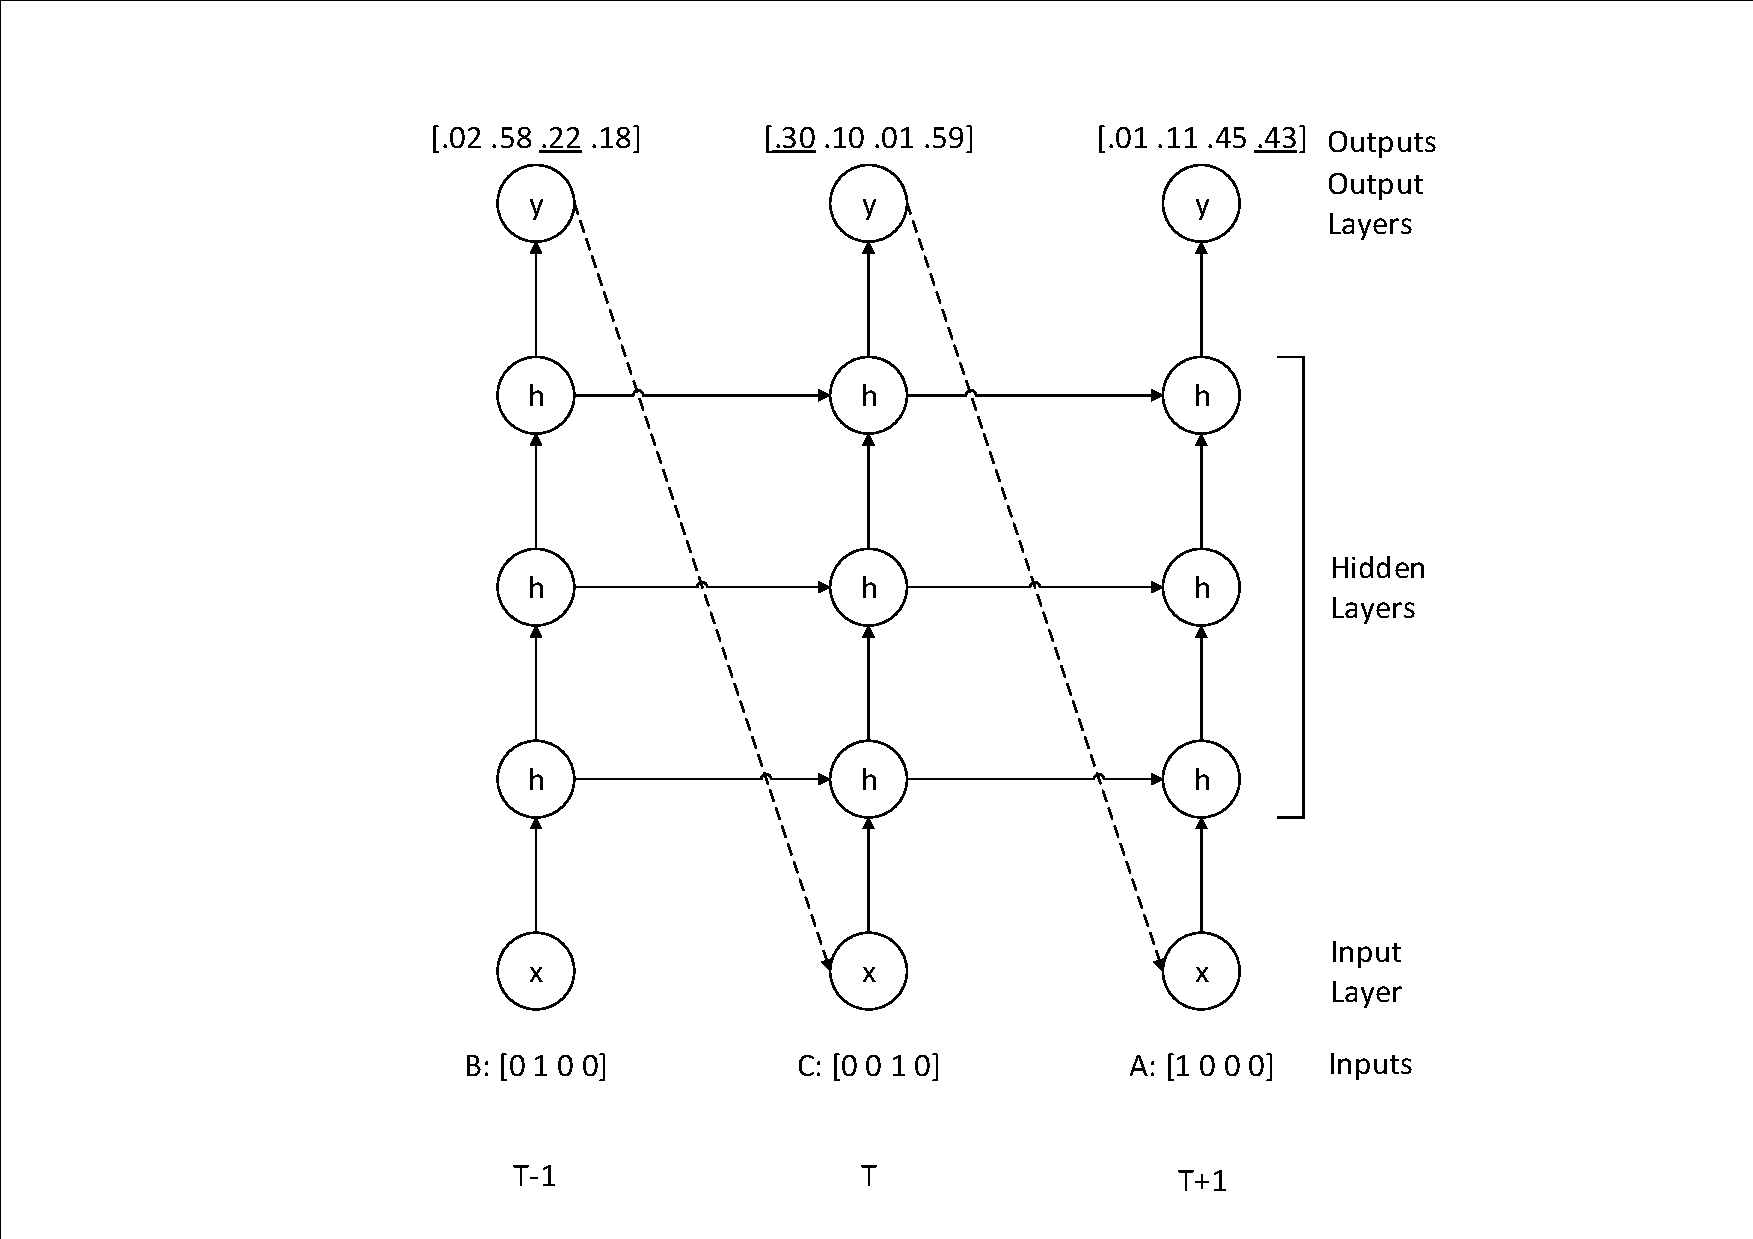
\includegraphics[width=\textwidth, trim = 4 4 4 4, clip, keepaspectratio]{images/char-rnn.pdf}
	\centering 
	\caption{Το μοντέλο \en{char-rnn}.}
	\label{fig:char-rnn}
\end{figure}

\subsection{\en{Model labeled-char-rnn}}

Το δεύτερο μοντέλο είναι επίσης ένα αναδραστικό νευρωνικό δίκτυο με 3 κρυμμένα επίπεδα στοιχείων \en{LSTM}. 
Εκτός απο ακολουθίες χαρακτήρων, το μοντέλο αυτό δέχεται και πληροφορία για το είδος του χαρακτήρα. 
Αντίστοιχα οι έξοδοί του, εκτός απο προβλέψεις για τον χαρακτήρα, περιέχουν και προβλέψεις για το είδος του χαρακτήρα. Με τον τρόπο αυτό θα εξετάσουμε κατά πόσο τα \en{RNN} μπορούν να εκμεταλλευτούν \en{a priori} γνώσεις για τον κώδικα. Σημειώνεται πως η συνάρτηση επιδόσεων αυτού το μοντέλου είνα γραμμικός συνδυασμός των επιμέρους επιδόσεων πρόβλεψης χαρακτήρα και είδους χαρακτήρα.

\begin{figure}[h]
	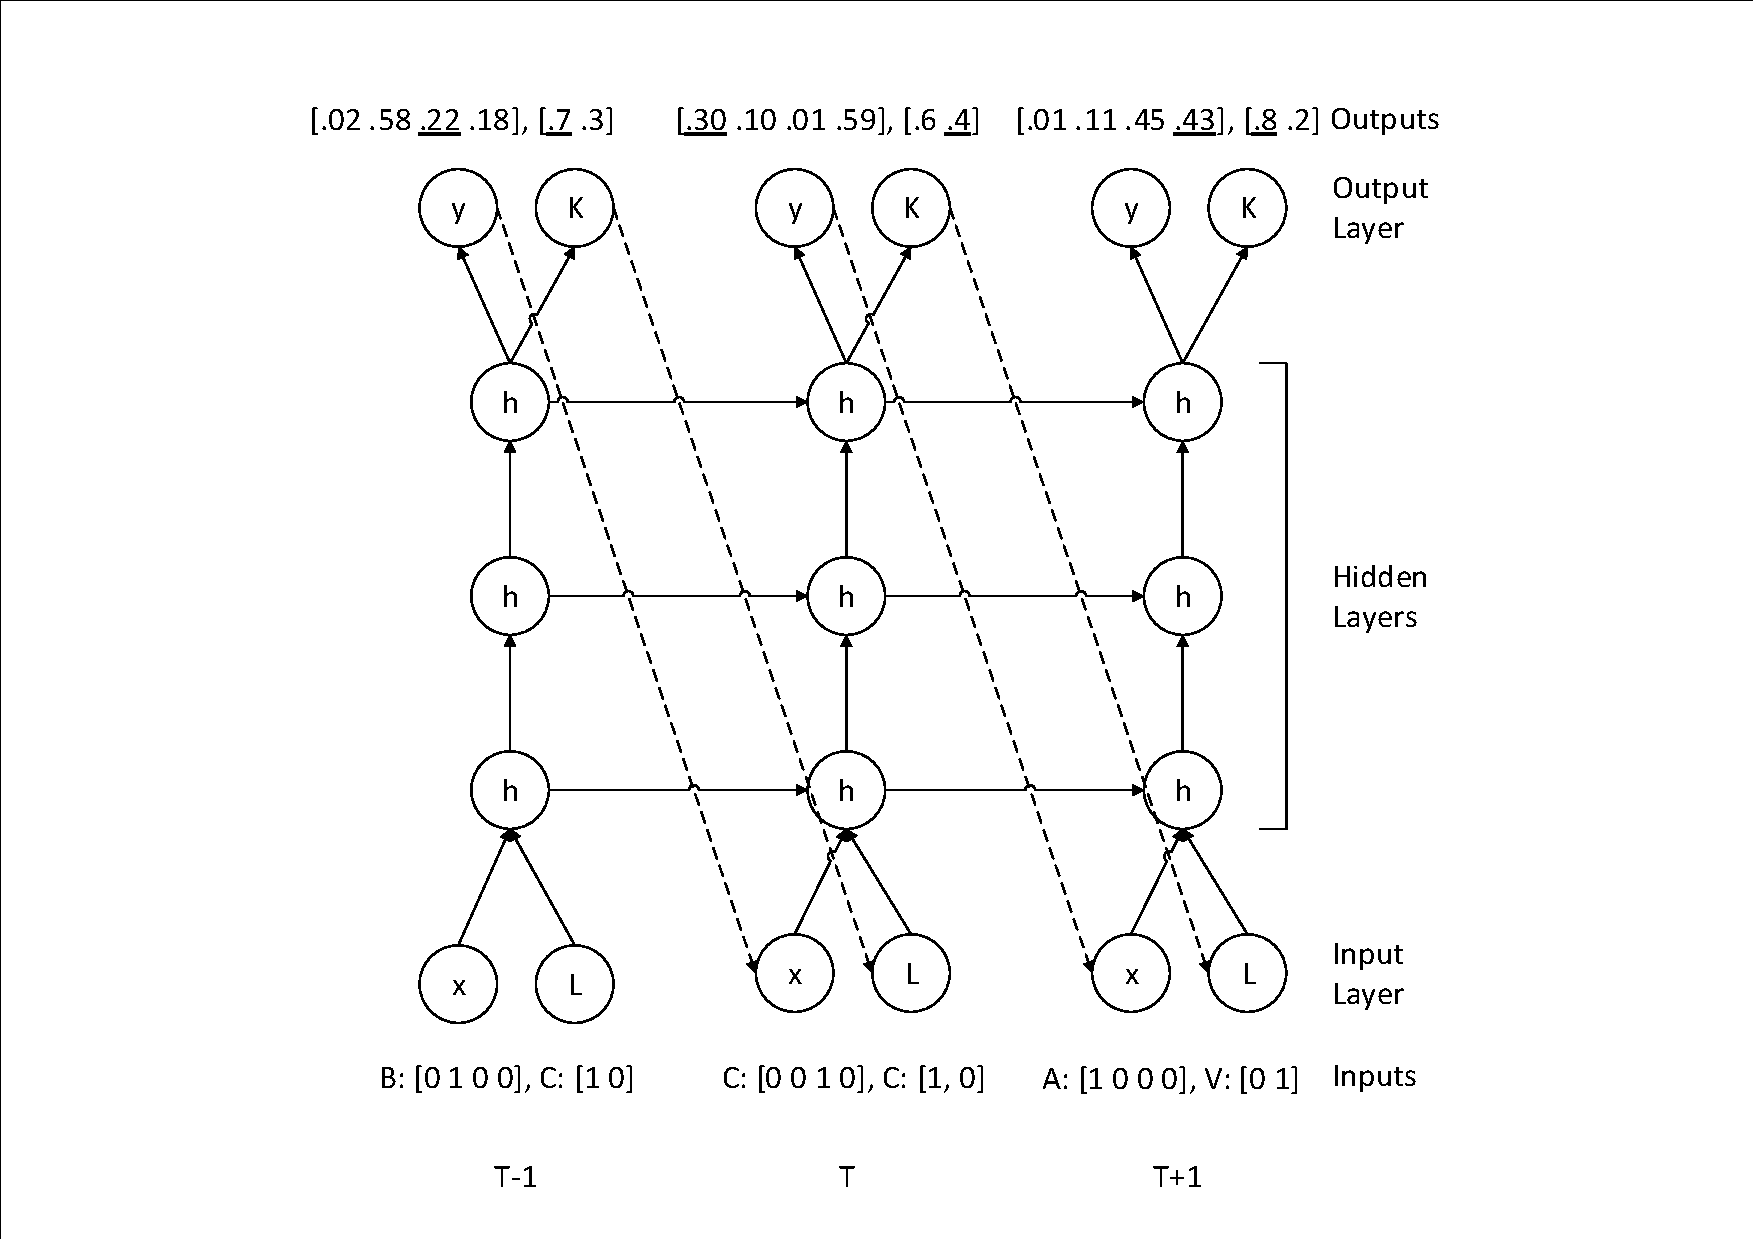
\includegraphics[width=\textwidth, trim = 4 4 4 4, clip, keepaspectratio]{images/l-char-rnn.pdf}
	\centering 
	\caption{Το μοντέλο \en{labeled-char-rnn}.}
	\label{fig:l-char-rnn}
\end{figure}

\section{\en{Pre-processing}}

Ο κορμός της διαδικασίας της προ-επεξεργασίας είναι ίδιος και για τα δύο σετ δεδομένων. 
Αρχικά αναζητούμε τα αρχεία με κατάληξη <<\en{.js}>> διασχίζοντας σειριακά όλους τους φακέλους των projects, εκτός απο αυτούς που αφορούν \en{testing} και \en{localization}.
Ο έλεγχος για το τελευταίο γίνεται απλοικά, ελέγχουμε δηλαδή αν οι φάκελοι φέρουν τα συνήθη ονόματα που χρησιμοποιούνται για τέτοιου είδους φακέλους.
Ο μη ενδελεχής έλεγχος καταφέρνει να αφαιρέσει την πλειοψηφία των επαναλαμβανόμενων αρχείων αφήνοντας ένα μικρό ποσοστό να περάσει.
Αυτό έχει ως αποτέλεσμα να εμπλουτιστεί η εκπαίδευση του νευρωνικού, χωρίς όμως να μονοπωλείται το ενδιαφέρον από αρχεία που περιέχουν τετριμμένο κώδικα.
Στη συνέχεια, με τη βοήθεια ενός εργαλείου ανάλυσης της σύνταξης και γραμματικής προγραμματιστικών γλωσσών (ονόματι \en{linguist}) προχωράμε στο περαιτέρω φιλτράρισμα αρχείων.
Συγκεκριμένα, εξαιρούμε αρχεία που έχουν την κατάληξη <<\en{.js}>> αλλα δεν είναι αρχεία κειμένου και αρχεία που είναι αυτόματα παραγώμενα και αποτελούν παραπροϊόν της διαδικασίας ανάπτυξης λογισμικού σε javascript.

Αφού επιλέξουμε τα αρχεία τα οποία θα αποτελούν το σετ δεδομένων μας προχωράμε στη διαδικασία της ελαχιστοποίησης του κώδικα (\en{minification, minimisation}).
Η ελαχιστοποίηση κώδικα, είναι η διαδικασία αφαίρεσης περιττών χαρακτήρων από των πηγαίο κώδικα, χωρίς να αλλάζει η λειτουργικότητά του. Τέτοιοι χαρακτήρες είναι τα κενά, τα σύμβολα αλλαγής παραγράφου, τα σχόλια και άλλα. Εδώ χρησιμοποίηθηκε το εργαλείο \en{jsmin}.
Με την επιλογή αυτή προσπαθούμε να αφαιρέσουμε την περιττή πληροφορία απο τα δεδομένα μας, ώστε να είναι πιο εύκολο για το μοντέλο να αποτυπώσει τις σημαντικές σχέσεις ανάμεσα στους δίαφορους χαρακτήρες.
Μετά το \en{minification} προσθέτουμε 2 ειδικούς χαρακτήρες για την αρχή και το τέλος κάθε αρχείου. Σημειώνεται πως θεωρούμε πως τα αρχεία ειναι \en{extended ASCII} κωδικοποιημένα και στην ουσία διαβάζουμε \en{bytes}. 

Για την εκπαίδευση του μοντέλου \en{labeled-char-rnn} χρειάζεται να προετοιμάσουμε με ανάλογο τρόπο την πληροφορία για το είδος των χαρακτήρων. Για το σκοπό αυτό χρησιμοποιούμε ένα άλλο εργαλείο ανάλυσης σύνταξης και γραμματικής προγραμματιστικών γλωσσών που φέρει το όνομα \en{pygments}.
Η επιλογή για τον διαχωρισμό των ειδών βασίζεται στα αυθαίρετα συντακτικά δέντρα \en{abstract syntax trees} της javascript, είναι όμως απλουστευμένη και δε χρησιμοποιεί δομές δέντρων, αλλά απλών διανυσμάτων.
Ο διαχωρισμός των χαρακτήρων γίνεται ανάμεσα στις ακόλουθες κλάσεις: \en{(\textbf{K}eyword, \textbf{N}umber, \textbf{R}egex, \textbf{S}tring, \textbf{O}perator, \textbf{P}unctuator, \textbf{I}dentifier).}

Οι χαρακτήρες και τα είδη τους αποθηκεύονται ως λίστες απο αλφαριθμητικά στοιχεία ώστε να είναι διαθέσιμα ανά πάσα στιγμή στην εκπαιδευτική διαδικασία.
Προφανώς υπάρχει χρονική αντιστοιχία μεταξύ των αρχείων που περιέχουν της ακολουθίες χαρακτήρων με τα αρχεία που περιέχουν το είδος κάθε χαρακτήρα, όπως στα παραδείγματα των πινάκων \ref{}, \ref{}. %TODO.
Συνηθίζεται σε τέτοιου είδους προβλήματα να <<ανακατεύονται>> οι ακολουθίες αλφαριθμητικών χαρακτήρων με σκοπό την γρηγορότερη/καλύτερη εκπαίδευση των μοντέλων.
Επειδή το ζητούμενο μας στη διπλωματική αυτή είναι η παραγωγή κώδικα και η σειρά των ακολουθιών είναι άρρικτα συνδεδεμένη με τη λειτουργικότητα και την ουσία των προγραμμάτων δεν προχωράμε σε αυτή την επιλογή.  

\begin{table}[]
\centering
\label{label-example}
\caption{Παράδειγμα αντιστοιχείας χαρακτήρων με το είδος τους σε μια ακολουθία}
\begin{tabularx}{\textwidth}{|l|XXXXXXXXXXXXXXXXXXXXX|}
\hline
\en{String 1} & \en{v} & \en{a} & \en{r} &   & \en{a} & = & 1 & \en{;} & \en{f} & \en{u} & \en{n} & \en{c} & \en{t} & \en{i} & \en{o} & \en{n} &   & \en{f} & \en{(} & \en{A} & \en{)} \\ \hline
\en{Label 1}  & \en{K} & \en{K} & \en{K} & \en{P} & \en{I} & \en{O} & \en{N} & \en{P} & \en{K} & \en{K} & \en{K} & \en{K} & \en{K} & \en{K} & \en{K} & \en{K} & \en{P} & \en{I} & \en{P} & \en{I} & \en{P} \\ \hline
\hline
\en{String 2} & \{ & \en{r} & \en{e} & \en{t}  & \en{u} & \en{r} & \en{n} &  & < & \en{o} & \en{k} &  > & \en{;} & \} & \en{c} & = & \en{f} & \en{(} & \en{1} &\en{0} & \en{)} \\ \hline
\en{Label 2}  & \en{P} & \en{K} & \en{K} & \en{K} & \en{K} & \en{K} & \en{K} & \en{P} & \en{S} & \en{S} & \en{S} & \en{S} & \en{P} & \en{P} & \en{I} & \en{O} & \en{I} & \en{P} & \en{N} & \en{N} & \en{P} \\ \hline
\end{tabularx}
\end{table}

\section{\en{Training}}


Η εκπαίδευση γίνεται στο \en{training set} του καθενός απο τα δύο σετ δεδομένων. 
Οι χαρακτήρες δίνονται ως \en{one-hot vectors} με διαστάσεις όσες και οι διαφορετικοί χαρακτήρες του σετ δεδομένων.
Χρησιμοποιείται η τεχνική του \en{dropout} και αλγόριθμος που χρησιμοποιείται για την ελαχιστοποίηση του λάθους είναι ο \en{TBPTT}.
Η συνάρτηση λάθους είναι η \en{cross-entropy loss function}: $\sum_x p(x) \log{q(x)}$, όπου $p(x)$ είναι η πραγματική κατανομή των χαρακτήρων και $q(x)$ η προβλεπόμενη κατανομή χαρακτήρων του μοντέλου.
Η συνάρτηση αυτή χρησιμοποιείται στην πλειοψηφία της σύγχρονης βιβλιογραφίας και εμπειρικά έχει καλά αποτελέσματα στην εκπαίδευση των αναδραστικών νευρωνικών δικτύων.
Εξίσου ευρεία χρήση συναντά και η συνάρτηση \en{rmsprop} που χρησιμοποιoύμε για τη βελτιστοποίηση του \en{gradient descent}.

%TODO Add some rmsprop reference 

Η εκπαίδευση του αναδραστικού νευρωνικού δικτύου γίνεται, πιο περιγραφικά ως εξής: δείχνουμε στο νευρωνικό δίκτυο ακολουθίες σταθερού μηκους, το οποίο προαποφασίζεται της εκπαίδευσης.
Ως αληθείς απαντήσεις δίνουμε ένα διάνυσμα ίσου μήκους με το προηγούμενο που περιέχει τους χαρακτήρες της επόμενης χρονικής στιγμής (κύλιση του διανύσματος κατά μία θέση).
Στην περίπτωσω του μοντέλου  \en{labeled-char-rnn} με όμοιο τρόπο δίνται και οι πληροφορίες σχετικά με το είδος των χαρακτήρων, μάζι με τους αντίστοιχους χαρακτήρες.
Με σκοπό την παραλληλοποίηση του προγράμματος, δίνουμε πολλά τέτοια παραδείγματα ταυτόχρονα.

Συνολικά εκπαιδεύουμε 4 διαφορετικά μοντέλα. Για κάθε dataset το αντίστοιχο \en{char-rnn} και \en{labeled-char-rnn} μοντέλο.
Για την εκπαίδευση των μοντέλων, πρέπει να αποφασιστεί ένα σύνολο παραμέτρων, που φέρουν σημαντική αξία για τις τελικές επιδόσεις του μοντέλου και την διάρκεια της εκπαίδευσης. Αυτές είναι:

\begin{itemize} 
\item Μήκος ακολουθίας \en{(Sequence length)}: Ο αριθμός χαρακτήρων που περιέχει μία ακολουθία.
\item Μέγεθος παρτίδας \en{(Batch size)}: Ο αριθμός των εκπαιδευτικών ακολουθιών που δίνονται παράλληλα στο μοντέλο.
\item Μέγεθους κρυμμένων επιπέδων \en{(Hidden state size)}: Ο αριθμός των στοιχείων \en{LSTM} που απαρτίζουν κάθε κρυφό επίπεδο.
\item Πιθανότητα \en{dropout}: Η πιθανότητα να κρατηθεί ένα στοιχείο στη διάρκεια τη εκπαίδευσης.
\item Αριθμός εποχών \en{(Epoch number)}: Ο αριθμός <<περασμάτων>> του τεστ δεδομένων.
\item Ρυθμός εκμάθησης \en{(Learning Rate)}: Πόσο γρήγορα μαθαίνει το σύστημα από τα λάθη του.

\end{itemize}

Για την στρατηγική επιλογής και την ακριβή τιμή των υπερ-παραμέτρων θα μιλήσουμε στο κεφάλαιο 5.

\section{\en{Inferring}}

Το μοντέλο που επιλέγουμε για καθένα απο τα πειράματα αποφασίζεται σύμφωνα με τις επιδόσεις του στην μετρική λάθους της εκπαίδευσης.
Για να είναι ευκολότερα ερμηνεύσιμα τα αποτελέσματα της εκπαίδευσης, θα χρησιμοποιούμε και την μετρική της <<ευστοχίας>>.
Η ευστοχία είναι το ποσοστό επιτυχημένων προβλέψεων επόμενου χαρακτήρα σε μία παρτίδα.

Η διαδικασία παραγωγης κώδικα που περιγράψαμε γενικεύεται και για τα μοντέλα που περιέχουν πληροφορία για το είδος των χαρακτήρων, δηλαδή δειγματοληπτούμε από την προβλεπόμενη κατανομή και χρησιμοποιούμε το αποτέλεσμα ως επόμενη είσοδο.
Μπορούμε να οδηγήσουμε, εν μέρει το σύστημα, αρχικοποιώντας το με κώδικα της επιλογής μας. Αυτό αλλάζει την εσωτερική κατάσταση του μοντέλου και το <<προϊδεάζει>> για το τι κώδικας μπορεί να ακολουθεί. 
Επιπρόσθετα, κατά τη διάρκεια της δειγματοληψίας έχουμε τη δυνατότητα να επηρεάσουμε την κατανομή που προτείνει το μοντέλο.
Αυτό ελέγχει το μοντέλο ως προς την <<σιγουριά>> του για τις προβλέψεις του και έχει τη δυνατότητα να κάνει τον παραγώμενο κώδικα είτε πιο ντετερμινιστικό είτε πιο ποικίλο.
Σημαντική ιδιότητα αυτής της προσθήκης είναι οτι δίνει στο μοντέλο τη δυνατότητα να ξεφύγει απο φαύλους κύκλους ντετερμινιστικών λαθών χάρη στην επιπλέον τυχαιότητας που εισάγεται.
Η συνάρτηση \en{Softmax Temperature}: 

\begin{equation}
P = \frac{e^{y/T}}{\sum_{k = 1}^{n} e^{y_k/T}}
\end{equation}

Όπου $P$ ειναι η νέα κατανομή, $y$ είναι η εξαγόμενη του νευρωνικού δικτύου πιθανοτικη κατανομή και $n$ ο αριθμός των διαφορετικών στοιχείων προς πρόβλεψη. $T$ είναι η τιμή της θερμοκρασίας που επηρεάζει την  κατανομή.
Για τιμές μεγαλύτερες του 1 ο κώδικας γίνεται πιο ποικίλος αλλα στο κόστος περισσότερων λαθών.
Τιμές μικρότερες του 1 έχουν ως αποτέλεσμα το σύστημα να είναι πιο σίγουρο για τις προβλέψεις του.



